\chapter{Custom Smart Actuator Module Design}
\label{ch:servomotor}

The performance of any articulated robotic system is strictly bound by the capabilities of its actuators.
In the context of the hexapod limb designed in Chapter \ref{ch:model}, the requirements for
trajectory tracking accuracy, and smoothness of motion are strict. While the geometric design dictates
the reachable workspace, the actuator dynamic dictates the quality of movement within that space.

To satisfy these requirements without incurring in the prohibitive costs of industrial-grade servomotors
(e.g. Dynamixel-X series \cite{robotis_dynamixel_x}), a custom actuator module was developed, aiming for a good
compromise between performance and cost. This section details the transition from analyzing the limitations of
standard low-cost components to the engineering of a high-performance, "smart" joint module.

\section{Limitations of Commercial Servos}
\label{sec:limitations}

The initial prototyping phase considered the use of the MG996R \cite{mg996r}, a ubiquitous standard-size
servomotor widely adopted in hobbyist robotics. However, a rigorous characterization revealed fundamental
limitations that rendered these units unsuitable for high-fidelity gait control.

The critical deficiencies, ranked by their impact on system performance, are:

\begin{itemize}
    \item \textbf{Feedback Sensor Degradation:} The internal feedback mechanism relies on a low-cost
        resistive potentiometer. Unlike non-contact solutions, this component involves a physical wiper
        sliding over a resistive track. Continuous operation leads to mechanical wear, causing progressive
        signal degradation and non-linearity. This deterioration was experimentally identified as the
        primary source of long-term positioning error.

    \item \textbf{Deadband and Stick-Slip Behavior:} To prevent motor hunting, the MG996R specifies a dead
        band width of $5\,\mu s$~\cite{mg996r}. When combined with the high static friction (stiction) of
        the metal gear assembly, this results in a significant effective dead-zone, making the joint fail
        to move for small command increments.

    \item \textbf{Limited Control Resolution and Bandwidth:} The standard PWM control protocol is inherently
        limited by the update rate. As per specifications, the MG996R operates on a $20\,ms$ period ($50\,Hz$
        frequency)~\cite{mg996r}. This low update frequency acts as a bottleneck for high-dynamic control loops,
        introducing a delay of up to $20\,ms$ between command and actuation.

    \item \textbf{Manufacturing Variability:} Significant unit-to-unit inconsistency was observed regarding
        the operational range characteristics. Two identical servos receiving the same PWM signal often
        align to different physical angles. This lack of repeatability makes the IK model unreliable without
        an intensive, individual calibration for each joint.

    \item \textbf{Obsolete Open-Loop Architecture:} Finally, as confirmed by the standard 3-pin interface
        (PWM, $V_{cc}$, GND)~\cite{mg996r}, these servos operate as "black boxes". The internal PID
        controller is hard-wired and inaccessible, preventing the implementation of advanced friction
        compensation or different control architectures in general. Crucially, the lack of feedback (current,
        real position, temperature) prevents any form of centralized Hardware-in-the-Loop control or online
        diagnostics.
\end{itemize}

To visualize and confirm the newly introduced limitations, an experimental characterization was performed
on two randomly selected units (Motor A and Motor B). The results, presented in Figure
\ref{fig:servo_deficiencies}, map the control signal pulse width ($T_{on}$) against the actual output
angle measured by a high-precision external magnetic encoder. The test involved a full sweep from $0.5\,ms$
to $2.5\,ms$ (Forward path, blue line) followed by a return to $0.5\,ms$ (Backward path, orange line).

\begin{figure}[htbp]
    \centering
    \begin{subfigure}[b]{0.48\textwidth}
        \centering
        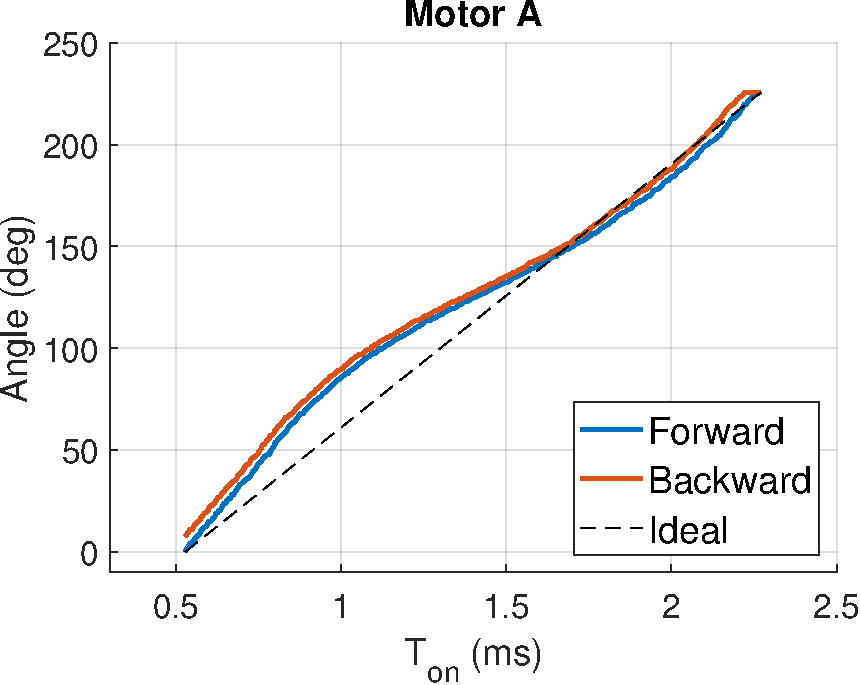
\includegraphics[width=\textwidth]{images/motor_char_A.pdf}
        \caption{}
        \label{fig:motor_A}
    \end{subfigure}
    \hfill
    \begin{subfigure}[b]{0.48\textwidth}
        \centering
        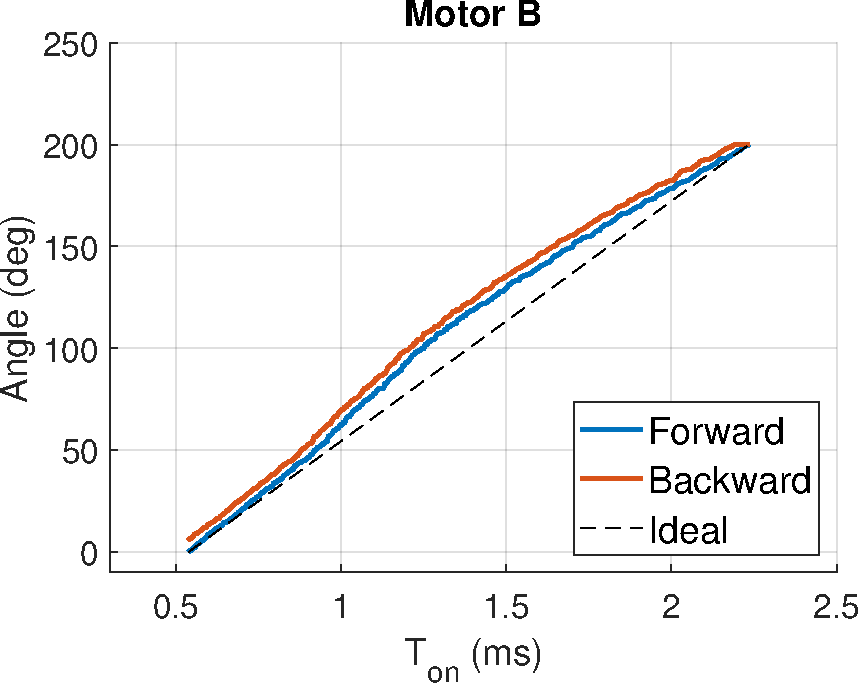
\includegraphics[width=\textwidth]{images/motor_char_B.pdf}
        \caption{}
        \label{fig:motor_B}
    \end{subfigure}
    \caption{Experimental Characterization of two MG996R Units.}
    \label{fig:servo_deficiencies}
\end{figure}

The dashed black line represents the ideal linear response ($Angle \propto T_{on}$) expected from a servomotor,
adjusted for the motor effective operative range. Both units show severe deviations from this ideal behavior,
introducing position errors exceeding $15^{\circ}$ thus making precise open-loop control impossible without a
complex, motor-specific calibration lookup table.

Furthermore, both plots exhibit a considerable hysteresis loop, visible as the vertical gap between the
forward and backward trajectories for the same PWM input.

Perhaps the most critical finding is the discrepancy between the two nominally identical units. Motor A covers
a range of approximately $0^{\circ}$ to $230^{\circ}$, while Motor B, driven by the exact same signal, spans a
smaller range from roughly $0^{\circ}$ to $200^{\circ}$. It should be noted that the graphs have been truncated
at the endpoints where a change in $T_{on}$ failed to produce any change in output position, indicating
mechanical or electronic saturation.

This inconsistencies confirms that a unified kinematic model cannot be applied to a robot using these actuators.
Each joint would require individual characterization and compensation, which is impractical for scalable
deployment.

Finally, although not visible at this macro-scale zoom, the stepped nature of the data acquisition
(confirmed during testing) revealed that the motors often remained stationary for input changes of
$5-10\,\mu s$ (corresponding to $1-2$ PWM step increments @$50\, Hz$), jumping only when the accumulated
error overcame the internal deadband and static friction.

Given these fundamental constraints, simply upgrading to a slightly more expensive hobby servo would yield
diminishing returns. The only viable solution was to redesign the control electronics entirely, retaining only
the mechanical shell and the DC motor, to create a fully programmable, closed-loop actuator.

\section{Hardware Design and Component Selection}
\label{sec:hardware}

The design of the custom actuator module is driven by a set of strict functional and physical requirements
derived from the limitations identified in the previous section.

The most critical requirement is maintaining the exact external form factor of the original servo. This
allows for a "drop-in replacement" into the existing hexapod limb structure without mechanical modification.
Consequently, all control electronics must be miniaturized to fit within the original motor chassis volume
(approx. $40 \times 20 \times 36$ mm).

The steady-state positioning error should ideally be reduced to $<\pm 0.5^{\circ}$ to enable precise
point-to-point gait control and the control interface could shift from a time-based PWM signal to a digital bus
protocol, enabling bi-directional communication (telemetry) and flexible control, while also simplifying
scalability.


\subsubsection{Position Feedback: Magnetic Encoder (AS5600)}

To eliminate the degradation issues of resistive potentiometers, the ams AS5600 \cite{as5600} magnetic rotary
position sensor was selected. This contactless sensor measures the orientation of a diametric magnet mounted
directly on the output shaft. Key advantages include:

\begin{itemize}
    \item \textbf{Contactless Operation:} Eliminates friction and mechanical wear, significantly extending
        the operational lifespan.
    \item \textbf{High Precision:} The sensor provides a 12-bit resolution over a full rotation,
        corresponding to a theoretical precision of $0.088^{\circ}$ per step ($360^{\circ}/4096$), which is
        well above the $0.5^{\circ}$ requirement.
    \item \textbf{Digital Interface:} It communicates via a robust $\text{I}^2\text{C}$ bus, reducing the
        susceptibility to electromagnetic noise inherent in analog ADC lines within the motor housing.
\end{itemize}


\subsubsection{Power Stage: H-Bridge Driver (DRV8870)}

To drive the DC motor, the DRV8870 \cite{drv8870} was chosen for its straightforward interface and integrated
protection features. Unlike the discrete transistor bridges often found in cheap servos, this integrated
H-bridge supports up to $3.6\,\text{A}$ peak current, comfortably handling the motor's stall current. The
driver allows for:

\begin{itemize}
    \item \textbf{Bi-directional Control:} Full forward/reverse driving via logic-level inputs and internal
        shoot-through protection, automatically handling the dead-time to prevent short circuits across the
        power rails during direction changes.
    \item \textbf{PWM Speed Control:} Compatible with high-frequency switching to reduce audible noise.
    \item \textbf{Integrated Protection:} Automatic current regulation (chopping) and thermal shutdown,
        protecting the electronics from stall conditions common in legged locomotion.
\end{itemize}


\subsubsection{Control Logic: Microcontroller (STM32F103C8T6)}

The "brain" of the module is the STM32F103C8T6 \cite{stm32f103c8t6}, a 32-bit ARM Cortex-M3 microcontroller.
This component was selected for its superior computational power ($72\,\text{MHz}$), necessary to execute the
real-time control algorithms, and for its comprehensive development ecosystem.

The key peripherals are the two $I^2C$ buses used for internal and external communication and interface:

\begin{itemize}
    \item \textbf{Internal Bus:} Dedicated high-speed channel for reading the AS5600 position sensor and
        interfacing with potential future on-board peripherals (e.g. EEPROM or current sensing).
    \item \textbf{External Bus:} The main interface for the actuator module. This will allows multiple
    servos to be daisy-chained on a single bus, eliminating the need for external PWM expansion boards (e.g.
    PCA9685) and simplifying the robot's wiring harness.
\end{itemize}

Additionally, the timer/PWM peripheral will accurately control the driver module.


\subsection{PCB Design and Layout}

All selected components, along with necessary passive elements (bypass capacitors, pull-up resistors, etc...),
were integrated into a custom-designed Printed Circuit Board (PCB). To respect the strict volume constraint,
the board was designed with specific dimensions to replace the original control board inside the servo case.
Additionally, an exposed 5-pin header provides access to the SWD interface (Serial Wire Debug), allowing for
firmware flashing and real-time debugging.

Detailed schematics of the board are provided in Appendix \ref{app:pcb} while the completed design can be seen
in Figures \ref{fig:pcb_layout} and \ref{fig:motor_result}. Note that provision was made for additional future
peripheral (e.g. current sensing), although outside the scope of the current experimental validation.

\begin{figure}[htbp]
    \centering
    \begin{subfigure}[b]{0.18\textwidth}
        \centering
        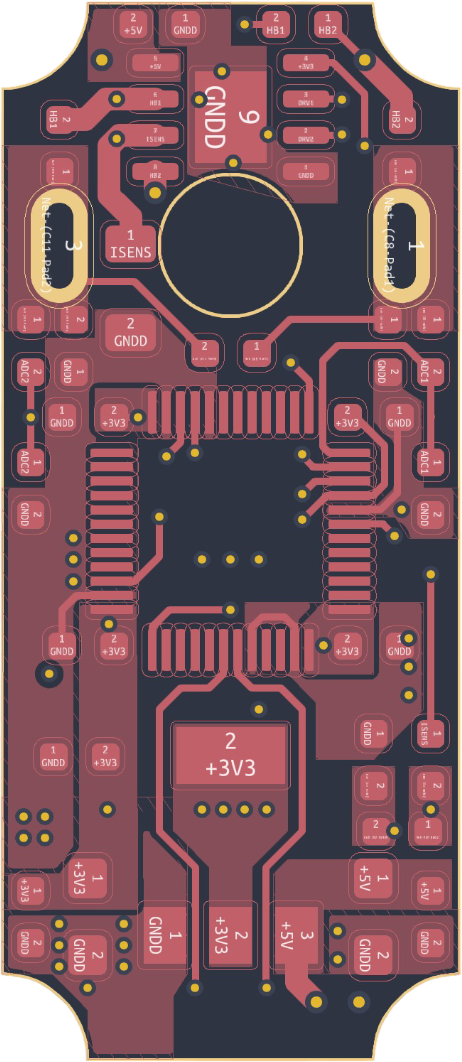
\includegraphics[width=\textwidth]{images/front_cad_pcb.png}
        \caption{CAD Front}
    \end{subfigure}
    \hfill
    \begin{subfigure}[b]{0.18\textwidth}
        \centering
        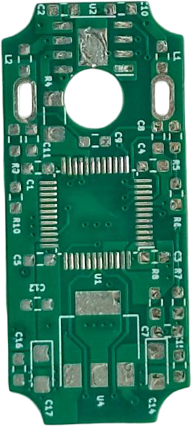
\includegraphics[width=\textwidth]{images/front_real_pcb.png}
        \caption{Real Front}
    \end{subfigure}
    \hfill
    \begin{subfigure}[b]{0.18\textwidth}
        \centering
        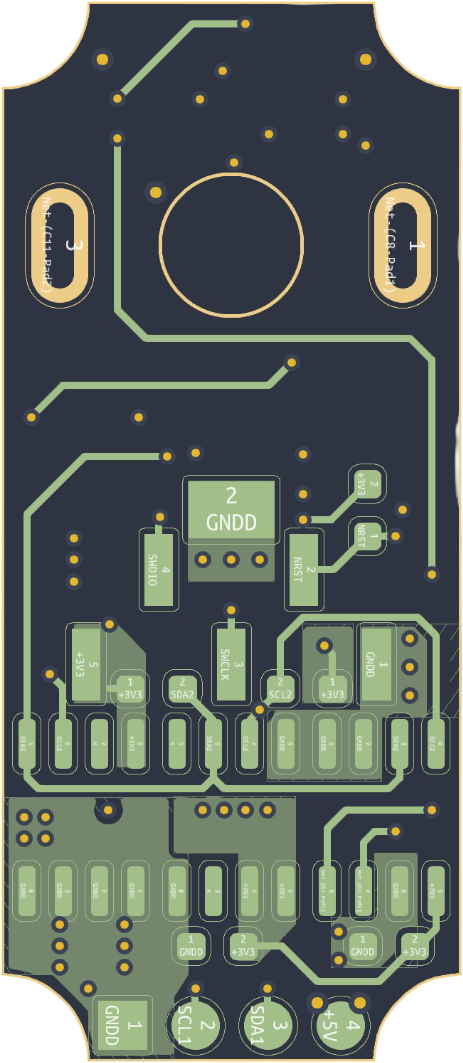
\includegraphics[width=\textwidth]{images/bottom_cad_pcb.png}
        \caption{CAD Bottom}
    \end{subfigure}
    \hfill
    \begin{subfigure}[b]{0.18\textwidth}
        \centering
        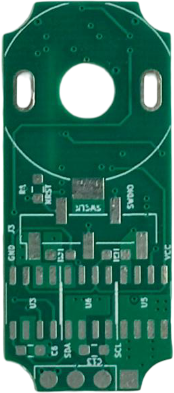
\includegraphics[width=\textwidth]{images/bottom_real_pcb.png}
        \caption{Real Bottom}
    \end{subfigure}
    \caption{Custom PCB Layout Design (CAD and Real).}
    \label{fig:pcb_layout}
\end{figure}

\begin{figure}[htbp]
    \centering
    \begin{subfigure}[b]{0.98\textwidth}
        \centering
        
\includegraphics[width=\textwidth]{images/front_motor.png}
        \caption{Front Side}
    \end{subfigure}

    \begin{subfigure}[b]{0.98\textwidth}
        \centering
        
\includegraphics[width=\textwidth]{images/bottom_motor.png}
        \caption{Bottom Side}
    \end{subfigure}
    \caption{Populated Custom PCB, i.e. Smart Actuator Internals.}
    \label{fig:motor_result}
\end{figure}
\section{Embedded Software Architecture}

The firmware running on the STM32 microcontroller was developed using a modular, object-oriented approach in
C++. This architecture ensures code reusability, encapsulation of hardware specifics, and ease of maintenance
and scalability. The software stack (Appendix \ref{app:software}) is organized into four distinct abstraction
layers, moving from low-level hardware management to high-level application logic.


\subsubsection{Layer 1: Vendor HAL}

The foundational layer consists of the Hardware Abstraction Layer (HAL) provided by the microcontroller
manufacturer. Modules such as \texttt{i2c.h} and \texttt{tim.h} handle the direct register-level configuration
of the MCU peripherals. Relying on these standard verified drivers ensures robust handling of interrupts and
basic I/O operations.


\subsubsection{Layer 2: Custom Middleware and Communication}

This layer acts as a bridge between the raw hardware and the high-level logic, abstracting the communication
protocols. Key modules include:

\begin{itemize}
    \item \textbf{I2C Device Wrappers:} Classes like \texttt{i2c\_device} and \texttt{i2c\_slave} extend the
        Vendor HAL to provide simplified interfaces for bus communication, handling read/write buffers and
        addressing logic.
    \item \textbf{Virtual Register:} This is the core component of the communication architecture. It
        implements the "Virtual Register Map" concept, abstracting the internal state of the actuator
        (positions, gains, modes) as a set of memory-mapped values. This allows the external master to
        interact with the servo seamlessly, as if reading from a standard memory device, changing its
        behaviour dynamically as needed.
\end{itemize}


\subsubsection{Layer 3: High-Level Component Drivers}

This layer contains the specific drivers for the chosen hardware components and the pure algorithmic logic,
independent of the specific MCU.

\begin{itemize}
    \item \textbf{Component Drivers:} The \texttt{AS5600} and \texttt{DRV8870} classes encapsulate the
        specific operational details of the sensor and driver. They utilize the lower layers to perform tasks
        such as reading raw magnetic angles or setting PWM duty cycles, exposing clean methods (e.g.
        \texttt{getAngle()}, \texttt{setSpeed()}) to the application layer.
    \item \textbf{Math and Control:} This module contains the implementation of the control algorithms,
        including the Switching PID logic. It is designed to be purely mathematical, accepting error inputs
        and producing control outputs without direct dependencies on hardware headers.
\end{itemize}


\subsubsection{Layer 4: Application Layer}

The highest level of the hierarchy integrates all previous modules to define the actuator's behavior.

\begin{itemize}
    \item \textbf{Smart Servo Class:} This main class encapsulates the entire logic of the actuator. It
        instantiates the drivers and control modules, managing the data flow between the sensor readings,
        the PID computation, and the motor output.
    \item \textbf{Entry Point:} The \texttt{main.cpp} and \texttt{CONFIG.h} files handle the system
        initialization, configuration, and the execution of the main real-time control loop.
\end{itemize}


\subsection{Control Strategy}

Achieving high-precision positioning in robotic joints is inherently challenging due to the presence of
nonlinear friction phenomena \cite{armstrong1994survey}, specifically static friction (Coulomb) and velocity
weakening effects (Stribeck). As extensively discussed in control literature, standard linear controllers like
the classical PID struggle to manage these non-linearities effectively.

In particular, the integral action required to overcome static friction often leads to overshoot. When
combined with the Stribeck effect, this energy imbalance prevents convergence to the setpoint, resulting in
persistent oscillations known as the "hunting phenomenon". While model-based control techniques could
theoretically compensate for these effects, they require precise parameter identification — which is difficult
to maintain over time due to wear and load changes — and impose a computational burden often incompatible with
low-cost embedded hardware.

A robust alternative that seems to mitigate these issues without requiring complex friction models is the
class of hybrid control strategies, such as Reset or Switching PID \cite{bisoffi2020stick, lorigiola2025switching}.
These approaches modify the internal state of the controller (specifically the integrator) based on discrete
logical rules triggered by the system's state (e.g. zero-crossing of the error or velocity).

The control strategy implemented in this custom actuator is directly derived from the Switching PID strategy
proposed and analyzed in \cite{lorigiola2025switching}. This approach uses a state-machine logic to
dynamically switch the integrator behavior and avoid hunting.

Since the rigorous mathematical derivation and stability proofs of this control strategy are extensive and already
well-documented in the referenced literature, they are considered outside the scope of this thesis. Instead,
this section provides a functional description of the algorithm and the pseudocode implementation specifically
tailored for the custom hardware application.


\subsubsection{Algorithm Description}

\begin{algorithm}[H]
    \footnotesize
    \caption{Switching PID for Friction Compensation}
    \label{alg:switching_pid}
    \begin{algorithmic}[1]
        \Require Reference $r_k$, Measurement $y_k$, Gains $K_p, K_i, K_d$
        \Ensure Control Input $u_k \in [-1, 1]$

        \State $e_k \gets r_k - y_k$ \Comment{Position Error}
        \State $v_k \gets \frac{y_k - y_{k-1}}{\Delta t}$ \Comment{Estimated Velocity}

        \vspace{0.1cm}

        % --- BLOCCO 1: PI Computation (Blu) ---
        \ColorBlock{RoyalBlue}{
            \textbf{1. PI Computation \& Anti-Windup} \\
            $\sigma \gets K_i \cdot e_k$ \\
            $\phi' \gets K_p \cdot (e_k + I_{state})$ \\
            $\phi \gets \text{Saturation of }\phi'$ \\
            $\Delta_{sat} \gets \phi' - \phi$ \\
            \textbf{if} $\text{sgn}(\sigma) == \text{sgn}(\Delta_{sat})$ \textbf{and} $\Delta_{sat} \ne 0$ \textbf{then} \\
            \hspace*{1.5em} $I_{state} \gets I_{state}$ \Comment{Hold integrator} \\
            \textbf{else} \\
            \hspace*{1.5em} $I_{state} \gets I_{state} + \sigma \Delta t$ \Comment{Update integrator} \\
            \textbf{end if}
        }

        \vspace{0.1cm}

        % --- BLOCCO 2: Switching Logic (Arancione) ---
        \ColorBlock{OrangeRed}{
            \textbf{2. Switching Logic} \\
            \textbf{if} $(\text{State} == \textsc{StickSlip}) \textbf{ and } (\sigma \cdot \phi \le 0)$ \textbf{then} \\
            \hspace*{1.5em} $\phi \gets -\phi$ \Comment{Reset energy} \\
            \hspace*{1.5em} $I_{state} \gets \frac{\phi}{K_p} - e_k$ \\
            \hspace*{1.5em} $\text{State} \gets \textsc{Overshoot}$ \\
            \textbf{else if} $(\text{State} == \textsc{Overshoot}) \textbf{ and } (v_k \cdot \phi \ge 0)$ \textbf{then} \\
            \hspace*{1.5em} $\phi \gets K_p \cdot \sigma / K_i$ \Comment{Restore linear behavior} \\
            \hspace*{1.5em} $I_{state} \gets 0$ \\
            \hspace*{1.5em} $\text{State} \gets \textsc{StickSlip}$ \\
            \textbf{end if}
        }

        \vspace{0.1cm}

        % --- BLOCCO 3: Output (Verde) ---
        \ColorBlock{ForestGreen}{
            \textbf{3. Output Calculation} \\
            $u_k \gets \text{Clamp}(\phi - K_d \cdot v_k, -1, 1)$
        }

        \vspace{0.1cm}

        \State \Return $u_k$
    \end{algorithmic}
\end{algorithm}

The control loop runs at a fixed frequency of $1\,\text{kHz}$. At each time step $k$, the algorithm described
in Algorithm \ref{alg:switching_pid} is executed.

The controller operates in two distinct logical states: when in \textbf{Stick-Slip State} (default) the
integrator is fully active to build up the torque necessary to overcome static friction ($F_s$). The logic
prioritizes "breaking out" of the stick phase. Detecting that the error has crossed zero (overshoot) triggers
the transition to the \textbf{Overshoot State}. In this mode, the logic serves to dampen the response by
inverting the control action, preventing the limit cycles (hunting) typical of high-gain PIDs on frictional loads.

The transition between these states is governed by the relationship between the generalized position error
($\sigma$) and the total proportional-integral control effort ($\phi$).

Notably, the term $\phi$ acts as a 'virtual' control effort that is reset discontinuously during state
transitions (Block 2), allowing the controller to instantly adapt its energy based on the
friction regime, a capability not present in standard linear PIDs.

This control strategy is originally derived for set-point regulation (point-to-point motion). While effective for
the quasi-static segments of the gait cycle, its application to dynamic trajectory tracking may require further
tuning or structural modifications (e.g. feed-forward terms). Addressing these specific dynamic tracking
optimization is considered outside the scope of this thesis and is left for future work.




\section{Module Characterization and Benchmarking}

The mechanical design and control strategy were validated by subjecting the custom actuator module to an
experimental characterization mirroring the one applied to to the commercial units in Section
\ref{sec:limitations} The tests were conducted using the integrated AS5600 magnetic sensor for feedback,
with the module powered at a nominal voltage of $6.7\,\text{V}$. The $\text{I}^2\text{C}$ bus was used to
transmit the target position directly as a 12-bit digital setpoint, bypassing the resolution limits of
standard PWM signaling.


\subsection{Static Analysis: Linearity and Hysteresis}

The first validation step focused on the static input-output relationship. A slow triangular ramp reference
($100\,ms$ per sensor LSB) spanning the full range in both Forward and Backward directions was administered
to the module. Figure \ref{fig:custom_linearity} illustrates the experimental results.

Compared to the commercial servo baseline (refer to Figure \ref{fig:servo_deficiencies}), the custom module
demonstrates significant visible improvements:

\begin{itemize}
    \item \textbf{Linearity:} The response closely follows the ideal characteristic $y=x$. The distortion,
        typical of the potentiometer-based commercial unit, is effectively eliminated.
    \item \textbf{Hysteresis Suppression:} The forward and backward paths are virtually indistinguishable at
        full scale. The removal of the mechanical potentiometer in favor of the non-contact magnetic sensor
        drastically reduces mechanical backlash, ensuring high repeatability regardless of the direction of
        approach.
    \item \textbf{Range Extension:} The operating range is no longer constrained by the physical limits of
        the potentiometer, granting access to the full $360^\circ$ of rotation. This continuous capability
        necessitates software phase unwrapping to ensure seamless transitions across the zero-crossing point.
\end{itemize}

\begin{figure}[htbp]
    \centering
    \begin{subfigure}[c]{0.48\textwidth}
        \centering
        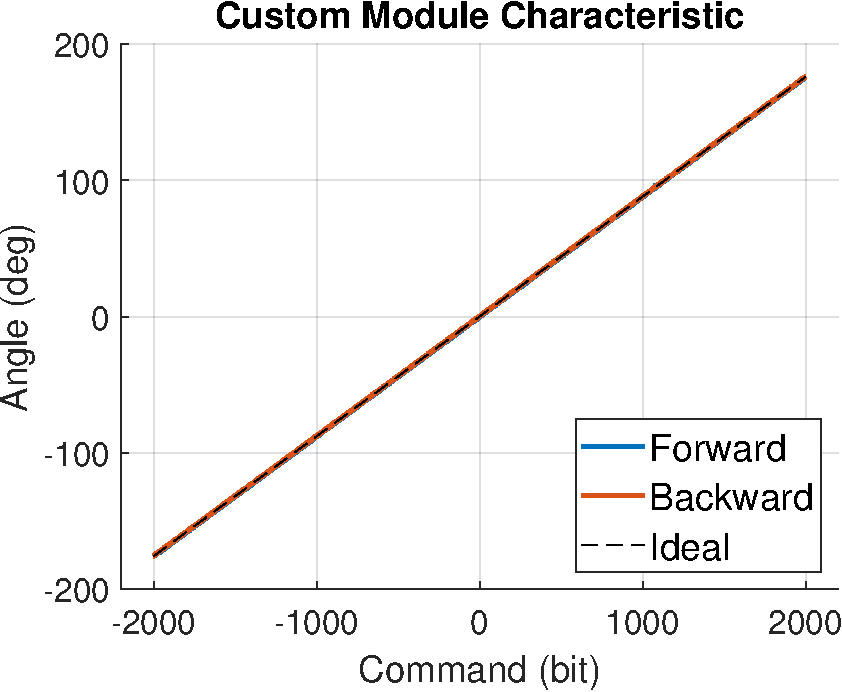
\includegraphics[width=\textwidth]{images/custom_linearity.pdf}
        \caption{Full-scale linearity analysis.}
        \label{fig:custom_linearity_full}
    \end{subfigure}
    \hfill
    \begin{subfigure}[c]{0.48\textwidth}
        \centering
        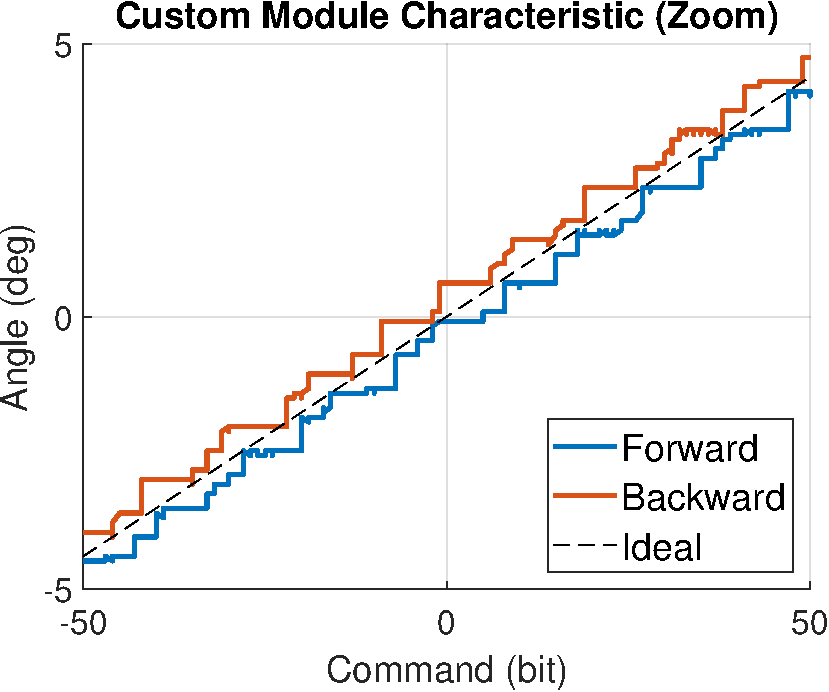
\includegraphics[width=\textwidth]{images/custom_linearity_zoom.pdf}
        \caption{Zoomed view showing micro-linearity.}
        \label{fig:custom_linearity_zoom}
    \end{subfigure}
    \caption{Input-Output Characteristic of the Custom Actuator.}
    \label{fig:custom_linearity}
\end{figure}


\subsection{Step Response Analysis: Sensitivity and Settling}

The module was then subjected to a series of step commands (square waves) of varying amplitudes: Micro-step
($1^\circ$), Mid-range ($15^\circ$), and Full-scale ($90^\circ$).

The results, presented in Figure \ref{fig:step_responses} and \ref{fig:step_error}, highlight two key behaviors:

\begin{itemize}
    \item \textbf{Resolution and Sensitivity ($1^\circ$):} Unlike the commercial unit, which exhibited a
        significant deadband preventing fine adjustments, the custom module responds reliably to micro-step
        commands as small as $1^\circ$ ($\approx 11$ LSB). Note that the visible jitter at this stage is sensor
        noise.
    \item \textbf{Transient Response ($15^\circ, 90^\circ$):} For larger transitions, the motor reaches the
        target setpoint rapidly. While a slight overshoot is visible, the system settles quickly without
        entering a limit cycle (hunting), validating the effectiveness of the Switching PID control algorithm.
\end{itemize}

\begin{figure}[htbp]
\centering
    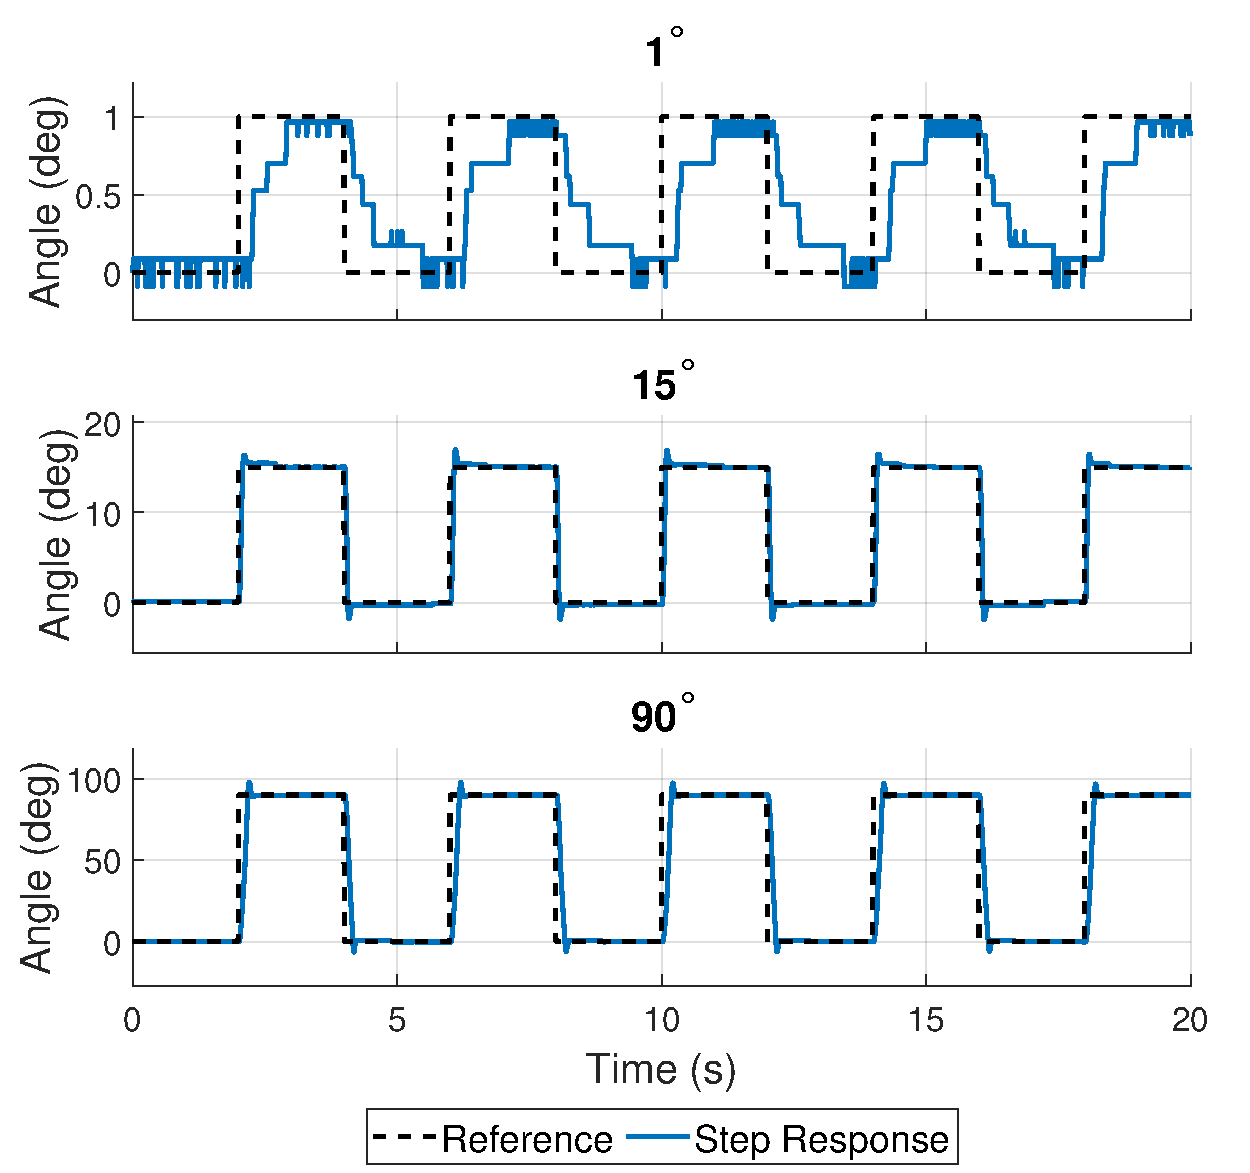
\includegraphics[width=0.98\textwidth]{images/custom_step_response_multi.pdf}
    \caption{Trajectory Tracking}
    \label{fig:step_responses}
\end{figure}

\begin{figure}[htbp]
    \centering
    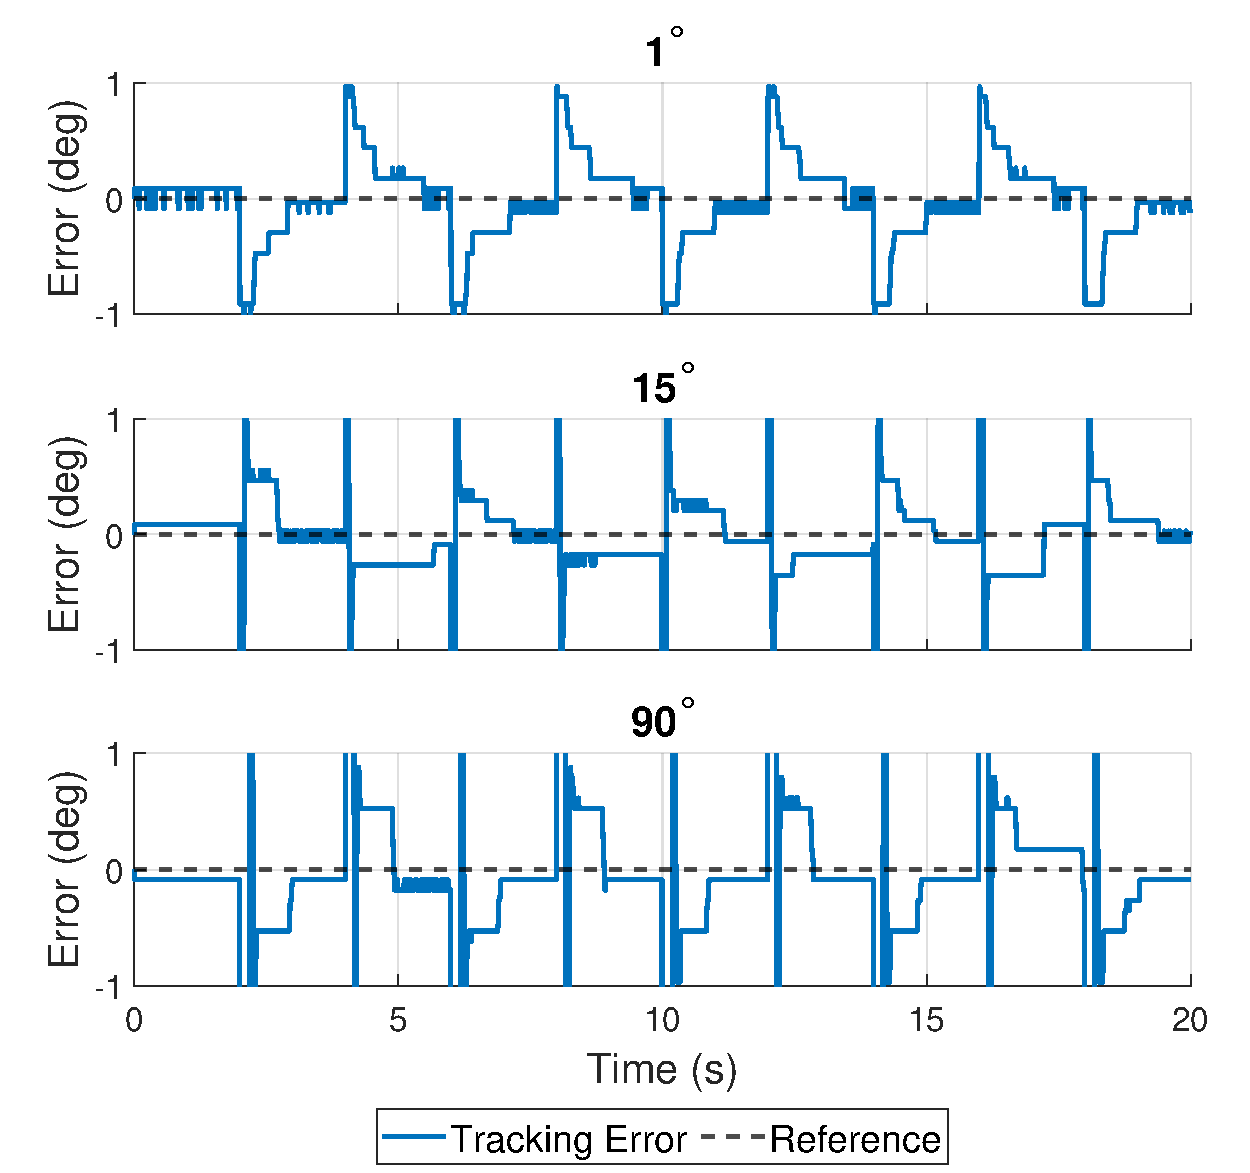
\includegraphics[width=0.98\textwidth]{images/custom_step_error_multi.pdf}
    \caption{Tracking Errors}
    \label{fig:step_error}
\end{figure}


\subsection{Results Summary}

The experimental results confirm that the custom actuator meets the strict requirements of the limb
application. The redesign has yielded a substantial increase in precision, accuracy, and controllability.
The transition to a digital interface ensures scalability and flexibility, while the mechanical form factor
remains compatible with the original design.

To quantify these improvements, a direct benchmark comparison was performed against the two commercial units
characterized in Section \ref{sec:limitations}. Figure \ref{fig:benchmark} illustrates the performance metrics
regarding positioning accuracy and mechanical play.

For the sake of brevity, the mathematical definitions of the metrics used in this analysis (RMSE, Absolute
Error, Hysteresis) are detailed in Appendix \ref{app:metrics}.

\begin{figure}[htbp]
    \centering
    
\includegraphics[width=0.96\textwidth]{images/final_benchmark.pdf}
    \caption{Performance Benchmark Results.}
    \label{fig:benchmark}
\end{figure}

The data reveals a dramatic enhancement in performance:

\begin{itemize}
    \item \textbf{Accuracy:} The Root Mean Square Error (RMSE), which serves as a reliable indicator of
        global linearity and tracking fidelity, dropped from an average of $\approx 14^{\circ}$ in the
        commercial units to just $\mathbf{0.37^{\circ}}$ in the custom prototype. This result comfortably
        satisfies the design requirement of $<\pm 0.5^{\circ}$ set in Section \ref{sec:hardware}.
    \item \textbf{Peak Error:} The Maximum Absolute Error was reduced from extreme values
        ($\approx 29^{\circ}$ for Unit A) to a manageable $\mathbf{1.49^{\circ}}$, effectively eliminating
        the macroscopic non-linearities observed in the analog potentiometers.
    \item \textbf{Hysteresis:} The stick-slip and backlash effects were significantly mitigated. The average
        hysteresis was reduced from $\approx 5^{\circ}$ to $\mathbf{0.65^{\circ}}$, validating the
        effectiveness of the Switching PID strategy in compensating for static friction.
\end{itemize}

Finally, a cost analysis (Appendix \ref{app:bom}) indicates that these performance gains were achieved within
a very limited budget, proving the viability of the proposed custom solution over expensive high-end commercial
alternatives. Further hardware and software improvements can be implemented in the next revision and are left
as future work.


